\documentclass{beamer}
\usepackage[utf8]{inputenc}
\usepackage[T1]{fontenc}
\usepackage[english,italian]{babel}
\usepackage{amsmath}
\usepackage{amssymb}
\usepackage{amsfonts}
\usepackage{mathrsfs}
\usepackage{graphicx}
\usepackage{wrapfig}
\usepackage{amsthm}
\usepackage{newlfont}
\usepackage{color}
\usepackage{natbib}
\usepackage{float}
\usepackage{textcomp}
\usetheme{Frankfurt}
\usecolortheme{beaver}
\usefonttheme[onlymath]{serif}
%\usetheme{CambridgeUS}

\setbeamertemplate{caption}{\raggedright\insertcaption\par}


\begin{document}
\title{\textcolor{black}{Analisi della complessità di reti neurali generate tramite algoritmi genetici}}
\author{Mattia Ceccarelli}
\date{A.A. 2017-2018 }
\institute{Corso di Laurea in Fisica \\ Università di Bologna}

\begin{frame}
 \maketitle
 Relatore: Dott. Enrico Giampieri
 
 Correlatore: Dott. Nico Curti
\end{frame}

\begin{frame}
 \frametitle{Introduzione}
 \begin{figure}
  \includegraphics[scale = 0.2]{images/TAC.png}
  \includegraphics[scale = 0.24]{images/convnn.png}
 \end{figure}

\end{frame}

\begin{frame}
 \frametitle{Reti Neurali: perceptron}
 \begin{figure}
   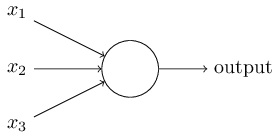
\includegraphics[scale = 0.5]{images/perceptron.png}    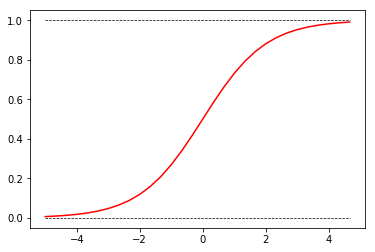
\includegraphics[scale = 0.35]{images/sigmoide.png}      
  \end{figure}
  A sinistra, rappresentazione di un perceptron in cui:
    \begin{equation*}
     output = f(\sum_{i = 1}^{n}x_{i}w_{i} + bias)   
    \end{equation*}
    A destra, la funzione di attivazione sigmoide definita come:  
    \begin{equation*}
      f(x) = \frac{1}{1 + e^{-x}}
    \end{equation*}
\end{frame}


\begin{frame}
\frametitle{Reti Neurali: MultiLayer Perceptron}
 \begin{figure}
  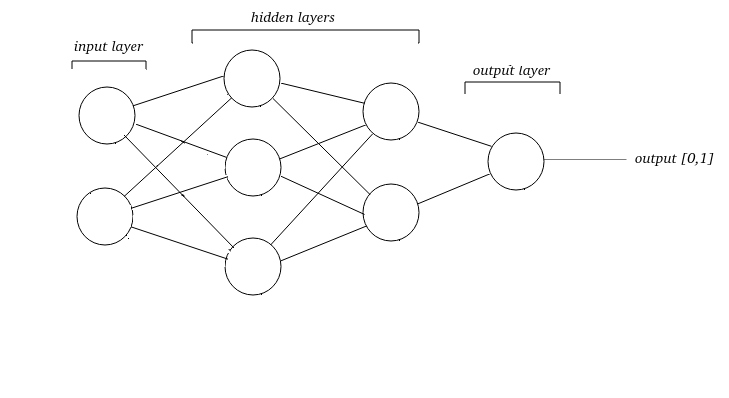
\includegraphics[scale = 0.4]{images/MLPClass.png}
 \end{figure}
 Un esempio di MultiLayer Perceptron semplice con 2 neuroni in input, 2 hidden layer con 3 e 2 neuroni ed un neurone in output.
 
 Il vettore di output del Layer i-esimo è dato da:
 $$\textbf{o}_i = f(W_{i,i-1}\cdot \textbf{o}_{i-1} + \textbf{b}_i)$$
 Dove $W_{ij}$ indica la matrice dei pesi tra il layer i-esimo e j-esimo

\end{frame}

\begin{frame}
 \frametitle{Algoritmi Genetici}
 \begin{figure}[H]
  \centering
  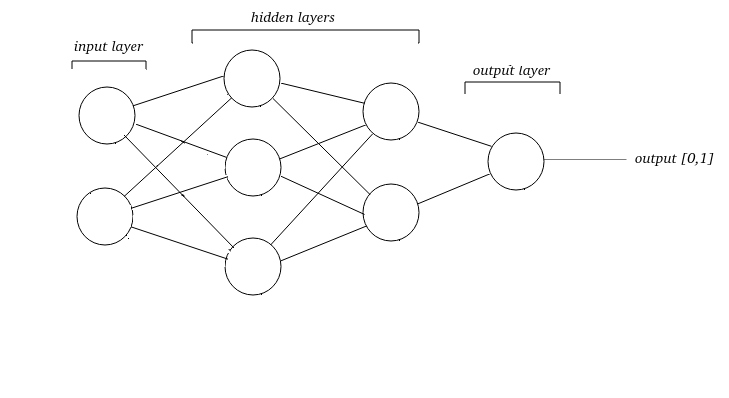
\includegraphics[scale = 0.2]{images/MLPClass.png}
  \caption{La rete precedente è identificata dal cromosoma [3,2]}
 \end{figure}

 \begin{figure}
  \includegraphics[scale = 0.27]{images/population.png}
  \includegraphics[scale = 0.31]{images/flow.png}
 \end{figure}
\end{frame}

\begin{frame}
 \frametitle{Funzione di fitness}
 \begin{enumerate}
  \item [-] la valutazione della rete avviene dopo l'addestramento, le due fasi avvengono in parti separate del dataset (train set e test set) 
  \item [-] Consente di selezionare gli individui migliori
  \item [-] Logarithmic Loss function consente di valutare l'incertezza della rete. È definita come:
 $$-log P(\frac{y_t}{y_p}) = -(y_t log(y_p) + (1-y_t)log(1-y_p))$$
 Dove:
 \begin{enumerate}
 \item[.] $y_t$ Classificazione corretta ($0$ o $1$)
 \item[.] $y_p$ Probabilità stimata che $y_t = 1$
 \end{enumerate}
 \end{enumerate}

\end{frame}

\begin{frame}
 \frametitle{Dataset}
 \begin{figure}
  \centering
  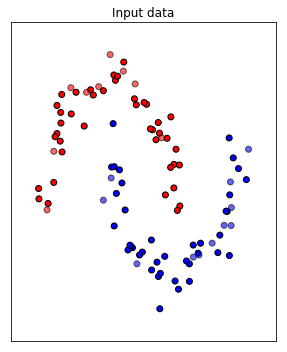
\includegraphics[scale = 0.5]{images/moons_noise.png}
  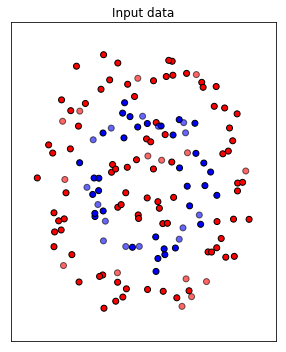
\includegraphics[scale = 0.5]{images/circles+_noise.png}
  \caption{\large A sinistra \textit{Moons} e a destra \textit{Circles+} con $noise = 0.2$.
  I dataset sono sintetici e il numero di punti è 100}
 \end{figure}

\end{frame}

\begin{frame}
 \frametitle{Classificazione su \textit{Moons}}
 \begin{figure}[H]
 \centering
 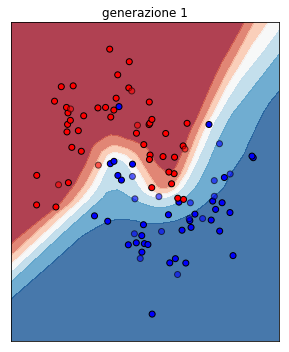
\includegraphics[scale = 0.25]{images/moons-rnd-log./1.png}
 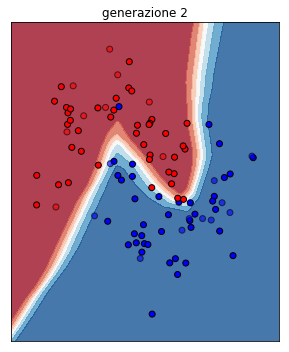
\includegraphics[scale = 0.25]{images/moons-rnd-log./2.png}
 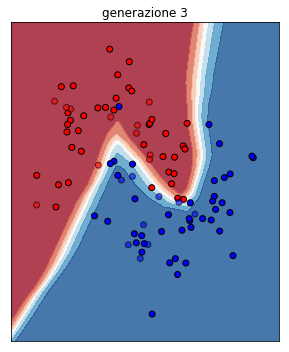
\includegraphics[scale = 0.25]{images/moons-rnd-log./3.png}
 \\
 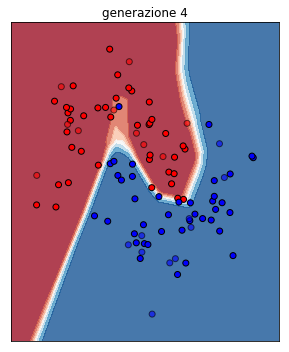
\includegraphics[scale = 0.25]{images/moons-rnd-log./4.png}
 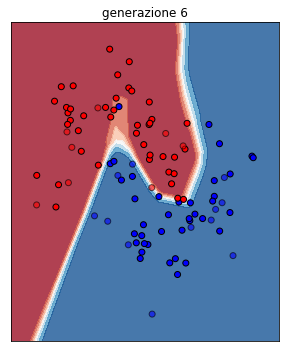
\includegraphics[scale = 0.25]{images/moons-rnd-log./5.png}
 \caption{\large Esempio di evoluzione nella classificazione di \textit{Moons}}
 \end{figure}
\end{frame}

\begin{frame}
 \frametitle{Classificazione su \textit{Circles+}}
 \begin{figure}
  \centering
  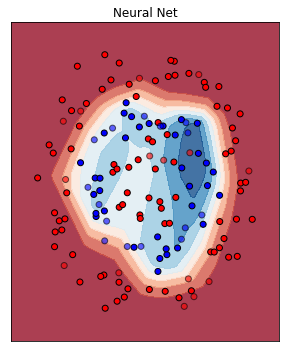
\includegraphics[scale = 0.25]{images/circle+-rnd-log./1.png}
  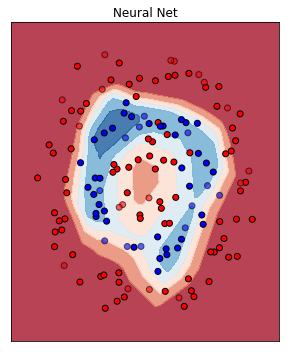
\includegraphics[scale = 0.25]{images/circle+-rnd-log./2.png}
  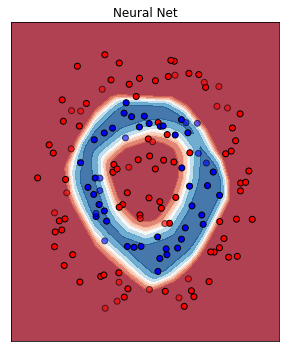
\includegraphics[scale = 0.25]{images/circle+-rnd-log./3.png}
  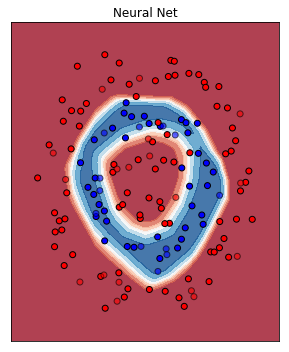
\includegraphics[scale = 0.25]{images/circle+-rnd-log./4.png}
  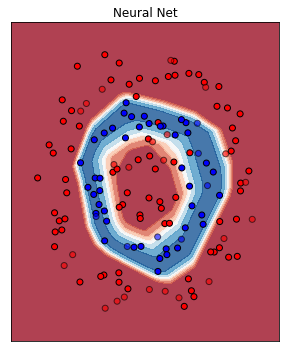
\includegraphics[scale = 0.25]{images/circle+-rnd-log./5.png}
  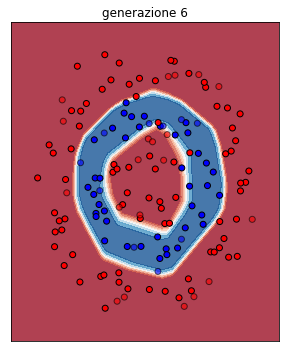
\includegraphics[scale = 0.25]{images/circle+-rnd-log./6.png}
  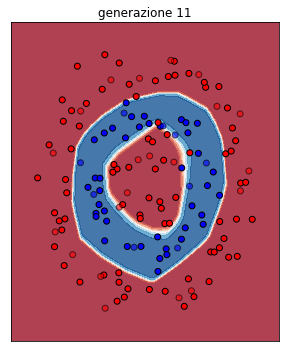
\includegraphics[scale = 0.25]{images/circle+-rnd-log./11.png}
  \caption{\large Esempio di evoluzione nella classificazione di \textit{Circles+}}
 \end{figure}   
\end{frame}

\begin{frame}
 \frametitle{Analisi della complessità}
 La rumorosità dei dataset modifica alcuni parametri della rete:
 \begin{enumerate}
  \item [-] Numero di collegamenti (Links)
  \item [-] Lunghezza (o profondità) ossia il numero di hidden layer 
  \item [-] Numero di neuroni nel layer più piccolo
 \end{enumerate}
 Per ognuno di essi sono state effettuate 70 run per dataset su 50 valori di noise compresi tra 0 e 1. 
 \\
 I grafici seguenti mostreranno media e deviazione standard.
\end{frame}

\begin{frame}
 \frametitle{Loss su \textit{Moons} e \textit{Circles+}}
  \begin{figure}[H]
   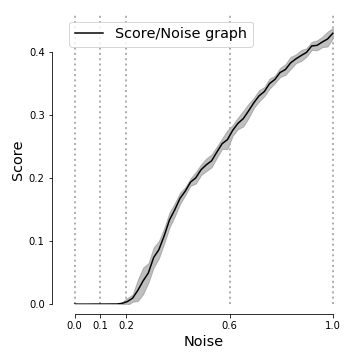
\includegraphics[scale = 0.42]{images/score_noise_moons.png}
   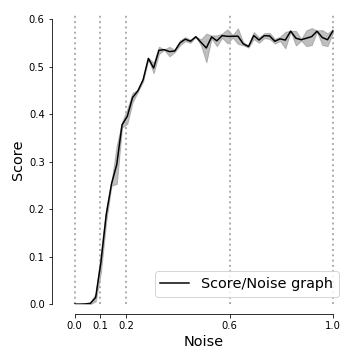
\includegraphics[scale = 0.42]{images/score_noise_circles+.png}
   \caption{\large Andamento dello score in funzione del noise in \textit{Moons} (a sinistra) e sul dataset \textit{circles+} (a destra)}
    \end{figure}

\end{frame}

\begin{frame}
 \frametitle{Links su \textit{Moons} e \textit{Circles+}}
 \begin{figure}
 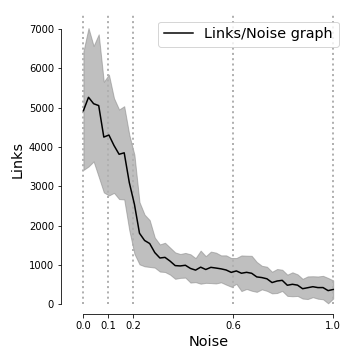
\includegraphics[scale = 0.42]{images/links_noise_moons.png}
 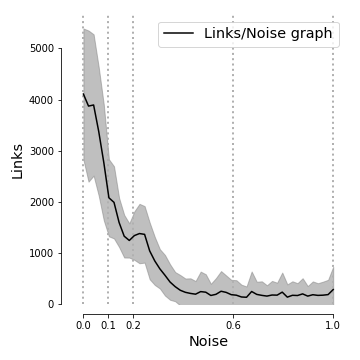
\includegraphics[scale = 0.42]{images/links_noise_circles+.png}
 \caption{\large Numero di collegamenti in funzione del noise su \textit{Moons} (a sinistra) e \textit{Circles+} (a destra)}
 \end{figure}
\end{frame}

% \begin{frame}
%  \frametitle{Links su \textit{Moons} e \textit{Circles+}}
%  \begin{figure}
%   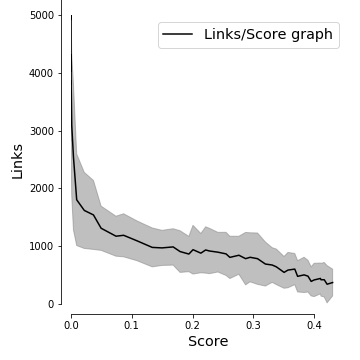
\includegraphics[scale = 0.42]{images/Links_Score_moons.png}
%   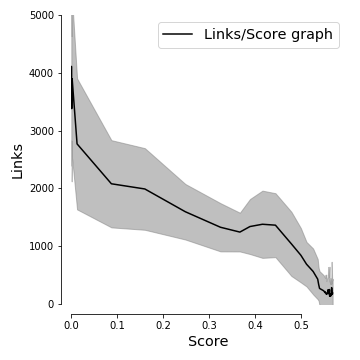
\includegraphics[scale = 0.42]{images/Links_Score_circles+.png}
%   \caption{\large Numero di collegamenti in funzione dello \textit{Score} sui dataset \textit{Moons} e \textit{Circles+}}
%  \end{figure}
 
 \begin{frame}
 \frametitle{Lunghezza}
 \begin{figure}
 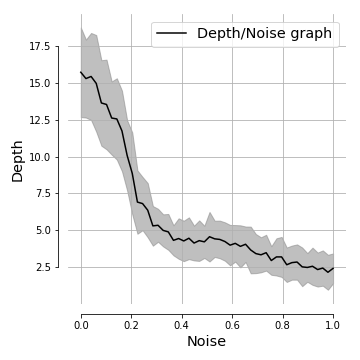
\includegraphics[scale = 0.42]{images/depth_noise_moons.png}
 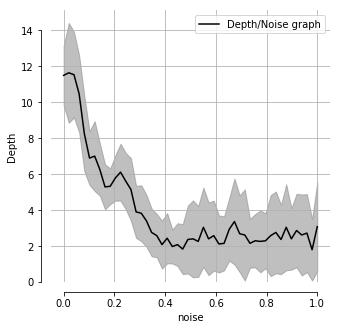
\includegraphics[scale = 0.42]{images/depth_noise_circles+.png}
 \caption{\large Numero di Hidden Layer della rete in funzione del noise su \textit{Moons} (a sinistra) e \textit{Circles+} (a destra)} 
 \end{figure}
\end{frame}

% \begin{frame}
%  \frametitle{Lunghezza}
%  \begin{figure}
%   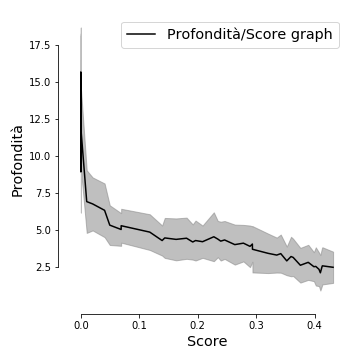
\includegraphics[scale = 0.42]{images/depth_Score_moons.png}
%   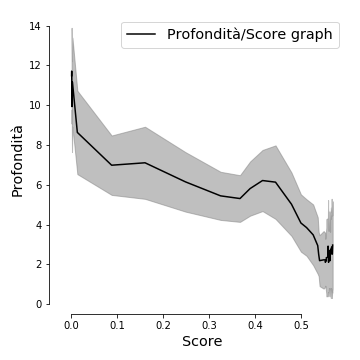
\includegraphics[scale = 0.42]{images/depth_Score_circles+.png}
%   \caption{\large Numero di layer della rete in funzione dello score su \textit{Moons} (a sinistra) e \textit{Circles+} (a destra)}
%  \end{figure}
% 
% \end{frame}

\begin{frame}
 \frametitle{Layer più piccolo della rete }
    \begin{figure}
    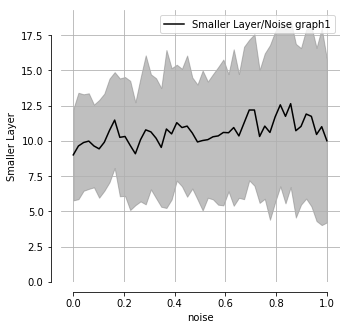
\includegraphics[scale = 0.42]{images/small_noise_moons.png}
    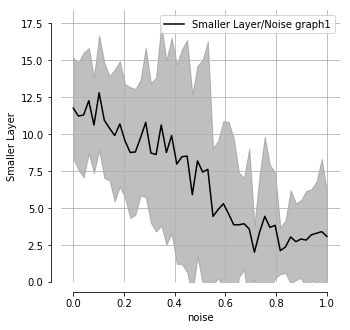
\includegraphics[scale = 0.42]{images/small_noise_circles+.png}
    \caption{\large Numero di neuroni nel layer più piccolo della rete su \textit{Moons} (a sinistra) e su \textit{Circles+} (a destra) in funzione del rumore}
 \end{figure}
\end{frame}

% \begin{frame}
%  \frametitle{Layer più piccolo della rete }
%     \begin{figure}
%     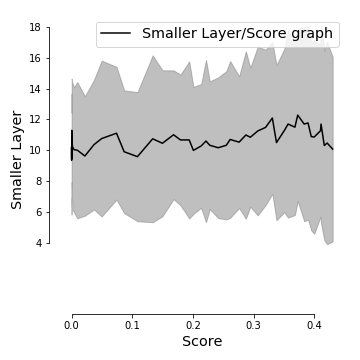
\includegraphics[scale = 0.42]{images/small_Score_moons.png}
%     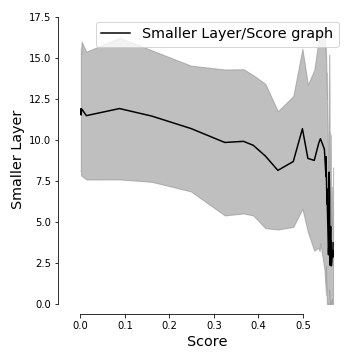
\includegraphics[scale = 0.42]{images/small_Score_circles+.png}
%     \caption{\large Numero di neuroni nel layer più piccolo della rete su \textit{Moons} (a sinistra) e su \textit{Circles+} (a destra) in funzione dello score}
%  \end{figure}
% \end{frame}


\begin{frame}
 \frametitle{Conclusioni}
 \begin{enumerate}
  \item [-] L'algoritmo è in grado di evolvere una popolazione e restituire una rete capace di classificare i dataset testati
  \item [-] La separazione tra train set e test set tra addestramento e valutazione della rete risulta sufficiente a far si che la complessità rimanga finita
 \end{enumerate}

\end{frame}

\begin{frame}
 \large
 \frametitle{Sviluppi Futuri}
 \begin{enumerate}
  \item [-] Applicazione a dataset reali
  \item [-] Applicazioni a reti neurali a convoluzione
  \item [-] Aggiunta nell'algoritmo di una penalità esplicita per reti troppo complesse e confronto dei risultati.
 \end{enumerate}

\end{frame}

\begin{frame}
\centering
 \huge Grazie per l'attenzione.
\end{frame}

\begin{frame}
 
\end{frame}

\begin{frame}
 \frametitle{Contents }
\end{frame}



\end{document}
